%
%---Beginning of Document---
%
% Use 1). latex recon-nim.tex, 2). dvipdfm recon-nim
%
%\RequirePackage{lineno}
\documentclass{elsart}
\usepackage[dvips]{color,graphics}
\usepackage[pdftex]{graphicx}
\usepackage{amssymb,amsmath}
%\setcounter{footnote}{0}
\setcounter{tocdepth}{5}
%
\usepackage{lineno} 
\linenumbers

\begin{document}
\begin{frontmatter}

\title{CLAS12 Event Reconstruction}

\author[JLab]{V. Ziegler\thanksref{corresponding}},
\author[JLab]{N. Baltzell},
\author[JLab]{D.S. Carman},
\author[INFN]{R. De Vita},
\author[JLab]{G. Gavalian},
\author[JLab]{V. Gyurjyan}, and
\author[JLab]{M.D. Mestayer}

\address[JLab]{Thomas Jefferson National Accelerator Facility, Newport News, VA 23606, USA}
\address[INFN]{INFN, Sezione di Genova, 16146 Genova, Italy}
\thanks[corresponding]{Corresponding author. Address: 12000 Jefferson Ave., Newport News, VA; 
e-mail: carman@jlab.org.}

\date{\today}

%\maketitle

\begin{abstract}
Abstract goes here
\end{abstract}

\end{frontmatter}

PACS:29.40.Mc \\
Keywords: CLAS12, event reconstruction
\newpage

\newpage
\tableofcontents

\vfil
\eject

\section{Reconstruction Framework and Tools}

\subsection{Clara}

\subsubsection{Service Composition}

\subsection{Common Tools}

\subsubsection{Packages and Functionalities}

\paragraph{Geometry}

\paragraph{Databases}

\paragraph{Plotting}

\paragraph{Analysis Tools}

\section{Data Formats}

\subsection{EVIO}

\subsection{HIPO}

\section{Monitoring and Calibration Suites}

\subsection{Framework}

\subsection{Data Monitoring}

\subsection{Calibration Suites}

The software programs used for the CLAS12 detector subsystem energy and time calibrations are
Java-based suites that employ the common tool developments discussed in Section~\ref{XX}. These
tools allowed for streamlined development of applications that are used across the different
subsystem suites including a COATJAVA calibration constant database interface, tools for detector
visualization, a data processing interface, and tools for fitting, plotting, and display with a standard
graphical user interface environment. Fig.~\ref{suites} shows representative screenshots of several
different CLAS12 subsystem calibration suites.

%%%%%%%%%%%%%%%%%%%%%%%%%%%%%%%%%%%%%%%%%%%%%%%%%%%%%%%%%%
\begin{figure}[htbp]
\vspace{4.5cm}
\begin{picture}(50,50) 
\put(55,-5)
{\hbox{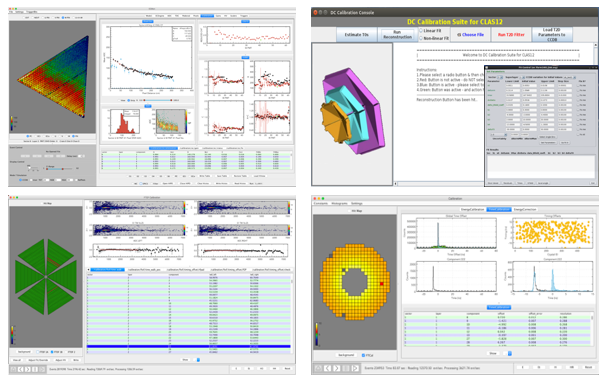
\includegraphics[width=1.0\textwidth,natwidth=610,natheight=642]{pics/suites.png}}}
\end{picture} 
\caption{Representative subsystem calibration code suites for ECAL~\cite{ecal-nim} (upper left),
  DC~\cite{dc-nim} (upper right), FTOF~\cite{ftof-nim} (lower left),  and FT~\cite{ft-nim} (lower right).}
\label{suites}
\end{figure}
%%%%%%%%%%%%%%%%%%%%%%%%%%%%%%%%%%%%%%%%%%%%%%%%%%%%%%%%%%%

The suites read in raw or reconstructed data files (from either beam data or Monte Carlo simulation output) in
either EVIO or HIPO data formats, display the various calibration quantities, fit the histograms to determine
the calibration constants, and then output the parameters into ASCII files that are compatible with the tables
defined in the CLAS12 Calibration Database (ccdb).

\section{Event Reconstruction}

\subsection{Introduction}

\subsection{Tracking Overview}

The event reconstruction software has been designed and developed within the ClaRA framework. The
reconstruction program must reconstruct, on an event-by-event basis, the raw data coming from either
simulation or the detectors to provide physics analysis output such as track parameters and particle
identification. Charged particle tracking is separated into the reconstruction of tracks in the central
(Silicon and Micromegas Vertex Trackers) and forward (Forward Micromegas Tracker and Drift
Chambers) detectors. The forward region covers the angular range from $5^\circ$ to $40^\circ$, while
the Central Detector covers approximately $40^\circ$ to $135^\circ$. In the central region a 5~T
solenoidal magnetic field bends charged tracks into helices, while forward-going tracks are bent by a
$\sim$2~T toroidal magnetic field. For both systems, track reconstruction comprises algorithms for
pattern recognition and track fitting. Hit objects, corresponding to the passage of a particle through a
particular detector component, require the transformation of an electronic signal into a location of the
track's position in the detector sub-system geometry. A hit is thus a geometric object, for example, a
line segment. These objects then form the input to the pattern recognition algorithms. This first step
involves the identification of clusters of hits and the determination of the spatial coordinates and
corresponding uncertainties for hits and clusters of hits. At the pattern recognition stage, hits that are
consistent with belonging to a trajectory (i.e. track) are identified. This set of hits is then fit to the
expected trajectory with their uncertainties, incorporating the knowledge of the detector material and
the detailed magnetic field map.

\subsubsection{Forward Tracking}

The Drift Chamber (DC) wire hit information is given by the wire geometrical location and the drift time
to the wire. Track-dependent corrections to the hit, such as left-right ambiguity and time-walk must then
be performed. Pattern recognition for the DC is done to first order on a "hit-based" basis. In hit-based
tracking, a hit is defined as a wire with a recorded signal.  No timing information is incorporated at the
preliminary stage of the reconstruction.  Uncorrelated hit noise in the DC are identified by a Simple Noise
Removal (SNR) algorithm and rejected. SNR stores all the data for a drift chamber layer (112 sense wires)
bitwise in an extended 128-bit word, with "set" bits corresponding to hits. The algorithm is configured
through parameters specifying the maximum tilt of a track segment and the number of missing layers
allowed in the formation of a segment. Using bitwise operations on the extended words, the algorithm
essentially operates as a parallel processor on all 112 sense wires in layer. This parallelism precludes the
need of a wire for-loop, enabling the algorithm to run in a negligible fraction of the total time for
reconstruction. More to the point, SNR actually saves time by reducing the combinations that must be
explored in the pattern-recognition phase of the ensuing track-finding. The hits remaining after the SNR
algorithm are grouped into clusters. 

Subsequent ``noise rejection'' algorithms are then applied to the clusters. These include the removal of the
interior hits from horizontal ``strings'' of hits along a layer~\footnote{The effectiveness of this cut follows
  from the observation that high-momentum tracks from hadrons typically cross the superlayers at a large angle,
  while ``curlers'' from low-momentum background follow curling trajectories with a significant part of the
  pattern being along layers.}, overlapping segments resolving, attached noise hits (resolved mostly using timing
information). The resulting trimmed clusters are then fit to a straight-line hypothesis, and those hits with
acceptable residuals are kept and identified collectively as a ``track segment''. 

Fits to the segments with a linear function serve as cluster refiners and are a preliminary step to estimating
a track trajectory. Track parameters are estimated in the local coordinate system of the chamber sector from
this trajectory.

Superlayers in a given region are linked a track segment is not a line but a plane.  Thus pairs of segments in
neighboring superlayers within one chamber (with superlayers of $\pm$6$^\circ$ stereo angle) represent the
intersection of two planes; that is a line.  This line's coordinates are evaluated midway between the two
superlayers, and is a 6-dimensional object (x,y,z and 3 angles) which we call a ``cross''. The first stage of
pattern-recognition consists of finding a track candidate, from a set of 3 crosses (1 each in R1, R2 and R3) that
are fit to a parabolic functional form to give us a ``track candidate''.

An additional  pattern reconstruction algorithm  matches of segments within even and odd superlayers to form
a track candidate where an entire superlayer can be missing by forming. The output of the pattern recognition
is a seed with initial parameters used to initialize the Kalman Filter.

Track fitting uses a Kalman Filter method with a 5-parameter track representation (x, y, tx, ty, q/p), defined
in a local coordinate system with the z-axis perpendicular to the chambers wire planes; where $tx=px$/$pz$,
$ty=py$/$pz$, in that frame~\cite{spiri} .  The equations of motion of the track in the torus field are solved u
sing a Runge-Kutta 4 numerical method.  The measurements used in the fit are the drift distances to the wires
taking into account the left/right position of the track with respect to the wire. Time corrections are applied
after hit-based tracking to account for the event start time, cable delays, propagation times along the wires,
event flight times to the hit location along the wires, beta-dependent corrections, and the effect of the magnetic
field on the cell isochrones which modify the drift times.  

After the times are corrected, the drift distance is computed using a tabulated distance-to-times
multi-dimentional arrays.  The drift distances are computed using a multi-dimentional interpolation method
using the segment local angle, the value of the magnetic field at the location of the hit and the corrected
times.  The Kalman fit is redone at time-based level using hits with corrected times and computed drift distances. 

A graphical representation of tracks in the CLAS Event Display is shown in figure~\ref{fig:dcTracks}.  The
display shows a longitudinal view of the chambers trapezoidal shapes. The field intensity is represented by a
color gradiant. The drift chamber hits correspond to the maroon shapes.  The bottom track goes through a
characteristic noise pattern in Region 1 (R1). Only the first superlayer in R1 is used to fit this track.  The tracks hit
the Forward Time-Of-Flight system and the Calorimeters.  The top track leaves a hit in the HTCC and is identified
as an electron. 

%%%%%%%%%%%%%%%%%%%%%%%%%%%%%%%%%%%%%%%%%%%%%%%%%%%%%%%%%%
\begin{figure}[htbp]
\vspace{4.5cm}
\begin{picture}(50,50) 
\put(55,-5)
{\hbox{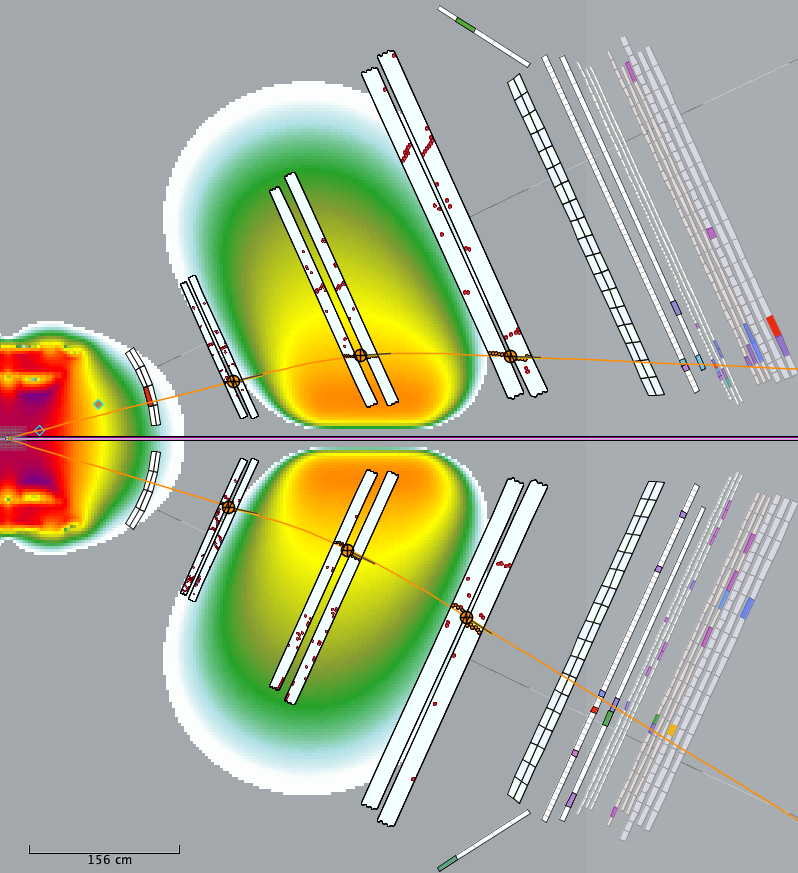
\includegraphics[width=1.0\textwidth,natwidth=610,natheight=642]{pics/dcTracks.png}}}
\end{picture} 
\caption{Event display of charged particle tracks in the Drift Chambers.}
\label{fig:dcTracks}
\end{figure}
%%%%%%%%%%%%%%%%%%%%%%%%%%%%%%%%%%%%%%%%%%%%%%%%%%%%%%%%%%%

\subsubsection{Central Tracking}

\subsubsection{Tracking Efficiency and Resolutions}

\subsection{Electromagnetic Calorimeters}

\subsection{Cherenkov Counters}

\subsubsection{High Threshold Cherenkov Counter}

\subsubsection{Ring-Imaging Cherenkov Counter}

\subsubsection{Low Threshold Cherenkov Counter}

\subsection{Time-of-Flight Systems}

For the CLAS12 Forward Time-of-Flight system (FTOF)~\cite{ftof-nim} and Central Time-of-Flight system
(CTOF)~\cite{ctof-nim}, the raw data from the detector elements readout during data acquisition that are
associated with a charged or neutral hit, include an ADC charge and hit time from a fitted flash ADC waveform
and a TDC time. The ADC and TDC information is recorded only for hits that are above the hardware readout
threshold. For hits in the FTOF and CTOF, the hardware thresholds for the flash ADC and discriminators are set
to be $\sim$1~MeV. During event reconstruction the ADC and TDC information are converted into deposited energy
and timing information after completion of the detector calibration procedures (see Refs.~\cite{ftof-nim,ctof-nim}
for calibration details). The measured hit times in each counter are related to the event start time defined with
respect to the appropriate RF beam bucket to determine the charged or neutral particle flight time.

\subsubsection{Reconstructed Hit Time}
\label{rec:time}

The reconstructed scintillation bar hit times need to account for the time delays along the readout path that
include the PMT signal transit time, the signal propagation times through the signal cables and the electronics, 
and any time-walk effects associated with the readout discriminators. For the FTOF readout, leading-edge
discriminators are employed, while for the CTOF readout constant fraction discriminators are employed and no
external time-walk corrections are required. The hit times reconstructed by the readout through the PMTs at
the left and right ends of each scintillation bar are given by:

\begin{equation}
t_{L/R} = (C_{TDC} \cdot TDC_{L/R}) - t_{L/R}^{walk} - \frac{C_{LR}}{2} + C_{p2p},
\end{equation}

\noindent
where $C_{TDC}$ is the TDC channel-to-time conversion factor (0.024~ns/bin), $TDC$ is the measured TDC value
relative to the trigger signal, $t^{walk}$ is the time walk function to correct for the pulse amplitude dependence of
the crossing times of the discriminator threshold, $C_{LR}$ is a time offset to center the left-right TDC difference
distribution about 0, and $C_{p2p}$ is a time offset to account for the different delay times along the signal path from
the photocathode of the PMT to the readout electronics. The paddle-to-paddle time offsets $C_{p2p}$ mainly account
for the different signal cable lengths.

The FTOF and CTOF particle hit times relative to the trigger signal can be determined separately from the times
$t_L$ and $t_R$ measured by the left and right PMTs of a given scintillation bar using:

\begin{equation}
t_{hit}^{L/R} = t_{L/R} - \frac{d_{L/R}}{v_{eff}},
\end{equation}

\noindent
where $d_{L/R}$ represents the distances along the bar from the hit point to the left and right PMTs given by
$d_{L/R}= L/2 \pm y$ with $y$ the hit coordinate along the bar and $L$ the counter length. The average hit time
is given by:

\begin{equation}
\bar{t}_{hit} = \frac{1}{2} ( t_{hit}^L + t_{hit}^R ) = \frac{1}{2} \left[ t_L + t_R - \frac{L}{v_{eff}} \right],
\end{equation}

\noindent
where $v_{eff}$ is the effective speed of light in the scintillation bar.

The hit coordinate along the bar is defined with respect to the center of the bar using:

\begin{equation}
  \label{tof-coor}
  y = \frac{v_{eff}}{2} (t_L - t_R - y_{offset}),
\end{equation}

\noindent
where $y_{offset}$ is an additional coordinate shift to center the coordinate distribution about zero.

In addition to the hit time determined from the TDC information associated with the left and right PMTs
from each counter of the FTOF and CTOF systems, a time is also derived from fitting the leading edge of
the flash ADC pulse shape. Due to the choice of fast timing PMTs for the detector readout and the use of
250~MHz FADCs, the number of samples on the leading edge of the PMT pulses is only 3 to 4, hence
the timing resolution is only $\sim$1~ns. In the event reconstruction of FTOF and CTOF hits, however, we
require that the hit times determined from the TDCs and from the FADCs match to within 10~ns to
reduce the probability of a mismatch of the ADC and TDC data for a given scintillation bar hit.

For CLAS12 flight time measurements, the event start time is determined by the FTOF system using the
path length $L$ determined from the forward drift chamber tracking by comparing the FTOF hit time
traced back to the vertex and linking this time to the closest RF pulse from the 499~MHz RF signal from
the accelerator. The timing residuals

\begin{equation}
  t_{res} = mod \left [ \left (\bar{t}_{hit} - \frac{L}{\beta c} \right) - \left (t_{RF} + \frac{z_v}{\beta_e c} \right),
    T_{RF} \right ]
\end{equation}

\noindent
are centered about zero. The reconstruction algorithm determines the event start time looking first for an
$e^-$ and then an $e^+$ in the ECAL. If none exists, then it looks for a high momentum $\pi^+$ or $\pi^-$. In
each case, if multiple candidates exist, the track with the highest momentum is chosen. In the expression for
$t_{res}$ above, $z_v$ represents the reconstructed event vertex from traceback of the drift chamber track
to the distance of closest approach to the defined beamline and $T_{RF}$ is the RF period. The term
$z_v/\beta_e c$ shifts the RF reference time to the event vertex. The modulus is employed as the RF time is a
pulse train with a period of $T_{RF}$. For the CTOF reconstruction, the flight time is computed as
$\bar{t}_{hit} - t_{ST}$.

\subsubsection{Reconstructed Hit Energy}
\label{rec:energy}

The reconstructed energy from the left and right ADC values of the PMTs for a given scintillator bar is given by:

\begin{equation}
E_{L/R} = (ADC_{L/R} - PED_{L/R}) \left [ \frac{\left( \frac{dE}{dx} \right )_{MIP} \cdot t}{ADC_{MIP}} \right ],
\end{equation}

\noindent
where $(ADC  - PED)$ is the measured pedestal-subtracted ADC integral, $ADC_{MIP}$ is the ADC value for normally
incident minimum-ionizing particles (MIPs) at the center of the scintillation bar, $\left( \frac{dE}{dx} \right)_{MIP}$
is the energy loss for MIPs in the scintillation bars (1.956~MeV/cm), and $t$ is the scintillation bar thickness.
The deposited energy is computed as the geometric mean of the deposited energy as determined from the left and
right PMTs $E_L$ and $E_R$ as $E_{dep} = \sqrt{E_L E_R}$.

\subsubsection{Hit Clustering and Matching}

A charged track incident upon the FTOF or CTOF can cross more than one scintillation bar. If there are multiple
scintillation bar hits associated with a single incident charged particle track, a hit cluster can be defined. These
clusters have associated with them a hit coordinate, energy, and hit time.

The $(x,y,z)$ coordinates assigned to a scintillation bar hit are given at the middle of the bar across its width
and depth, and from eq.(\ref{tof-coor}) along the counter length. Hits are assigned as part of a cluster if they
fall within a matching distance of the charged track projected from the drift chambers to the FTOF counters
using a straight line extrapolation or from the Central Vertex Tracker to the CTOF counters following the
helical trajectory in the solenoid field. This matching distance is $\pm$1 counter about the hit scintillation bar
and $\pm$10~cm along the counter length.

With hit clusters defined, the associated cluster coordinate is defined as the energy-deposited weighted average.
The deposited energy of the cluster hit is the energy sum of the cluster hits and the hit time is the energy-deposited
weighted average. Note that in both the FTOF and CTOF systems, the maximum cluster size is $N=2$.

For the FTOF system in the range of polar angles from 5$^\circ$ to 30$^\circ$ where two parallel scintillation
bar planes are included (referred to as panel-1b - closest to the target, and panel-1a - farthest from the target)
(see Ref~\cite{ftof-nim}), the hit time is assigned as the time resolution weighted average of the two cluster times
after evolving the panel-1a hit to the location of the panel-1b hit using the path length determined from the
extrapolated drift chamber track. The combined plane hit time is given by:

\begin{equation}
t_{comb} = \dfrac{ t_{1b}^{cluster} {\delta_{1b}}^{-1} + (t_{1a}^{cluster} - \Delta r/\beta) {\delta_{1a}}^{-1}}
           {\left( {\delta_{1b}}^{-1} + {\delta_{1a}}^{-1} \right)},
\end{equation}

\noindent
where $\delta_{1b/1a}$ are the measured counter effective time resolutions, $t_{1b/1a}^{cluster}$ are the cluster
hit times, and $\Delta r/\beta$ is the path length from the panel-1a hit location to the panel-1b hit location for
the track of speed $\beta$.

As the effective FTOF time resolutions for the panel-1b counters are in the range from $60-110$~ps and those
for the panel-1a counters are in the range from $90-160$~ps, the combined plane hit time resolution is $\sim$20\%
better than that for the panel-1b hit time resolution. If there is a panel-1b (panel-1a) hit without an associated
panel-1a (panel-1b) hit, the hit time is defined solely by the panel-1b (panel-1a) hit.

\subsection{Central Neutron Detector}

\subsection{Forward Tagger}

\subsection{Event Builder}

\subsubsection{Particle Identification Performance}

\section{Data Processing}

\subsection{Data Processing Workflow}

\subsection{DSTs and Analysis Trains}

\subsection{Computing Tools}

\subsection{Resources}

\section{Code Management}

\subsection{Repositories}

\subsection{Releases}

\subsection{Unit Tests}

\subsection{Code Validation Suites}

\section{Conclusions}

\ack

This work was supported in part by DOE Contract DE-AC05-84ER40150.

\begin{thebibliography}{99}

\bibitem{clas12-nim}
V.D. Burkert {\it et al.}, ``The CLAS12 Spectrometer at Jefferson Laboratory'', to be published in Nucl.
Inst. and Meth. A, (2020). (see this issue)

\bibitem{ftof-nim}
D.S. Carman {\it et al.},   ``The CLAS12 Forward Time-of-Flight System'', to be published in Nucl.
Inst. and Meth. A, (2020). (see this issue)

\bibitem{ctof-nim}
D.S. Carman {\it et al.}, ``The CLAS12 Central Time-of-Flight System'', to be published in Nucl.
Inst. and Meth. A, (2020). (see this issue)

\bibitem{ecal-nim}
G. Asryan {\it et al.}, ``The CLAS12 Forward Electromagnetic Calorimeter'', to be published in Nucl.
Inst. and Meth. A, (2020). (see this issue)

\bibitem{dc-nim}
M.D. Mestayer {\it et al.}. ``The CLAS12 Drift Chamber System'', to be published in Nucl. Inst. and
Meth. A, (2020). (see this issue)

\bibitem{ft-nim}
M. Battaglieri {\it et al.}, ``The CLAS12 Forward Tagger System'', to be published in Nucl. Inst. and
Meth. A, (2020). (see this issue)

\bibitem{spiri}
Alexander Spiridonov, Optimized Integration of the Equations of Motion of a Particle in the HERA-B Magnet

\end{thebibliography}

\end{document}
